\chapter{Implementación de CitaLab}
\label{chap:implementacion}

\section{Organización del código}

CitaLab está desarrollado con Python en el backend y React y TypeScript en la
interfaz. El paquete separa la agenda, los perfiles, las políticas, los agentes
y la evaluación. Esta organización permite que las tres arquitecturas utilicen
los mismos datos y herramientas. La Tabla~\ref{tab:modulos} resume las
responsabilidades de cada módulo.

\begin{table}[!htbp]
\centering
\caption{Módulos del prototipo.}
\label{tab:modulos}
\small
\begin{tabularx}{\textwidth}{L{0.25\textwidth}Y}
\toprule
\textbf{Módulo} & \textbf{Responsabilidad} \\
\midrule
\texttt{domain/agenda} & Simulador FHIR: \texttt{Slot}, \texttt{Appointment} y \texttt{CommunicationRequest}. Reserva, cancelación, reprogramación y recordatorio con versiones, bloqueo e idempotencia. \\
\texttt{domain/profiles} & Atributos con procedencia y resolución por finalidad. \\
\texttt{domain/policy} & Reglas \texttt{CMP-*} con referencias normativas y red de seguridad de emergencias. \\
\texttt{assistant/tools} & Capa de herramientas, propuestas y confirmación. \\
\texttt{assistant/schemas}, \texttt{prompts} & Contratos de salida e instrucciones versionadas de cada rol. \\
\texttt{assistant/respond} & Planes de respuesta, textos deterministas y comprobaciones de redacción. \\
\texttt{assistant/engine} & Motor de turnos y arquitecturas M5 (LangGraph), S1 y H. \\
\texttt{llm/client} & Cliente único para Groq y Gemini: JSON Schema estricto, llamadas a funciones, reintentos y trazas. \\
\texttt{evaluation/*} & Escenarios, usuario simulado, oráculo, runner, análisis y revisión ciega. \\
\texttt{portal/*} & API FastAPI, sesiones, almacenamiento SQLite y servicio de la interfaz. \\
\bottomrule
\end{tabularx}
\end{table}

\section{Simulador HIS y alcance FHIR}

La agenda utiliza un subconjunto de FHIR R4 para representar pacientes,
agendas, huecos, citas y recordatorios \citep{fhirR4}. Cada recurso conserva
una versión que cambia al modificarse. El simulador comprueba la propiedad de
la cita, su estado y la disponibilidad del destino antes de aplicar una operación.

Las escrituras se realizan bajo un bloqueo. Si la solicitud ya se ejecutó con
la misma clave de idempotencia y los mismos parámetros, se devuelve el resultado
guardado. Reutilizar esa clave para una operación distinta produce un rechazo.
Así, repetir una petición no crea una segunda reserva.

En una reprogramación se comprueba el destino antes de liberar el hueco de
origen. Si el nuevo horario ya no está disponible, se conserva la cita. Los
recordatorios se representan mediante recursos \texttt{CommunicationRequest}
marcados como simulados. Guardarlos no envía mensajes fuera de CitaLab.

\section{Contratos de los agentes}

Los agentes devuelven objetos JSON definidos mediante modelos Pydantic. El
cliente transforma estos contratos en esquemas y valida las respuestas recibidas.
Los campos admiten valores nulos cuando falta información y las enumeraciones
limitan las acciones que se pueden proponer.

El contrato de contexto recoge veinte campos, entre ellos intención, servicio,
fecha, cita referida, idioma y renuncia al perfil. El coordinador de M5 utiliza
cinco campos para indicar la acción, la cita, el hueco, el dato pendiente y el
motivo. Los contratos completos están en el repositorio público del trabajo
(apartado~\ref{sec:metodo-ejecucion}).

Si el proveedor rechaza el esquema estricto, el cliente solicita un objeto JSON
con una guía de campos y lo valida localmente. Una respuesta que no cumple el
contrato admite una reparación con el error de validación. Si tampoco se puede
utilizar esa respuesta, el asistente aplica el respaldo previsto para la tarea.

\section{Estado de la conversación}

Cada conversación conserva la tarea pendiente y la información aportada por la
persona. Incluye la operación, el servicio, las fechas, la cita seleccionada,
las opciones mostradas y la propuesta pendiente. También guarda el idioma,
las preferencias de la conversación, la renuncia al perfil y el último recibo.

Los mensajes sucesivos completan o corrigen esos datos. Pedir otro horario
modifica la propuesta, pero no la confirma. Elegir una opción de una lista
tampoco autoriza la escritura. El diseño prevé actualizar la tarea cuando la
persona inicia otra gestión y retirar las restricciones que ya no corresponden.
La campaña encontró casos en los que una consulta conservó un filtro anterior
(apartado~\ref{sec:caso-filtro}), por lo que esta actualización no siempre
funcionó como se había previsto. Los ajustes limitados a un turno caducan al
terminar ese turno.

\section{Recorrido de una reserva}

Una reserva comienza con la interpretación del mensaje. Si faltan el servicio
o las condiciones necesarias para buscar, el asistente pregunta por ellos.
Cuando dispone de esos datos, consulta los huecos compatibles y presenta las
opciones. Las preferencias autorizadas pueden cambiar su orden.

Al elegir un hueco se prepara una propuesta con los datos de la cita. La agenda
todavía no cambia. En un turno posterior, la persona puede confirmar, corregir
o descartar la propuesta. La confirmación activa las comprobaciones de acceso,
vigencia y disponibilidad. Solo después se registra la reserva y se genera un
recibo con los datos del resultado.

En M5 participan los agentes según la fase de la gestión. En S1, un mismo agente
elige las llamadas a herramientas. En H, el código fija la secuencia. La
confirmación y la operación sobre la agenda son comunes a las tres variantes.

\section{Portal CitaLab}

El portal permite conversar con el asistente y consultar los datos sintéticos.
El equipo investigador puede elegir además la arquitectura y el proveedor de
cada conversación. Las propuestas aparecen en tarjetas desde
las que se pueden confirmar o descartar (Figura~\ref{fig:portal-propuesta}).
Si la persona cambia de opinión antes de confirmar, la propuesta pendiente se
sustituye por una nueva revisión, y solo se puede confirmar la vigente.
La persona también puede ajustar sus preferencias para el turno o la
conversación y confirmar cambios del perfil.

Los controles visibles permiten revisar y aceptar la propuesta, pero no
sustituyen las garantías del servidor. Antes de escribir se comprueban la
autorización, la vigencia y la disponibilidad, y la operación aplica la clave
de idempotencia. Una propuesta visible no reserva el hueco ni garantiza que
siga disponible al confirmar.

\begin{figure}[!htbp]
\centering
\setlength{\fboxsep}{0pt}%
\begin{minipage}[t]{0.45\textwidth}
\vspace{0pt}
\fcolorbox{black!25}{white}{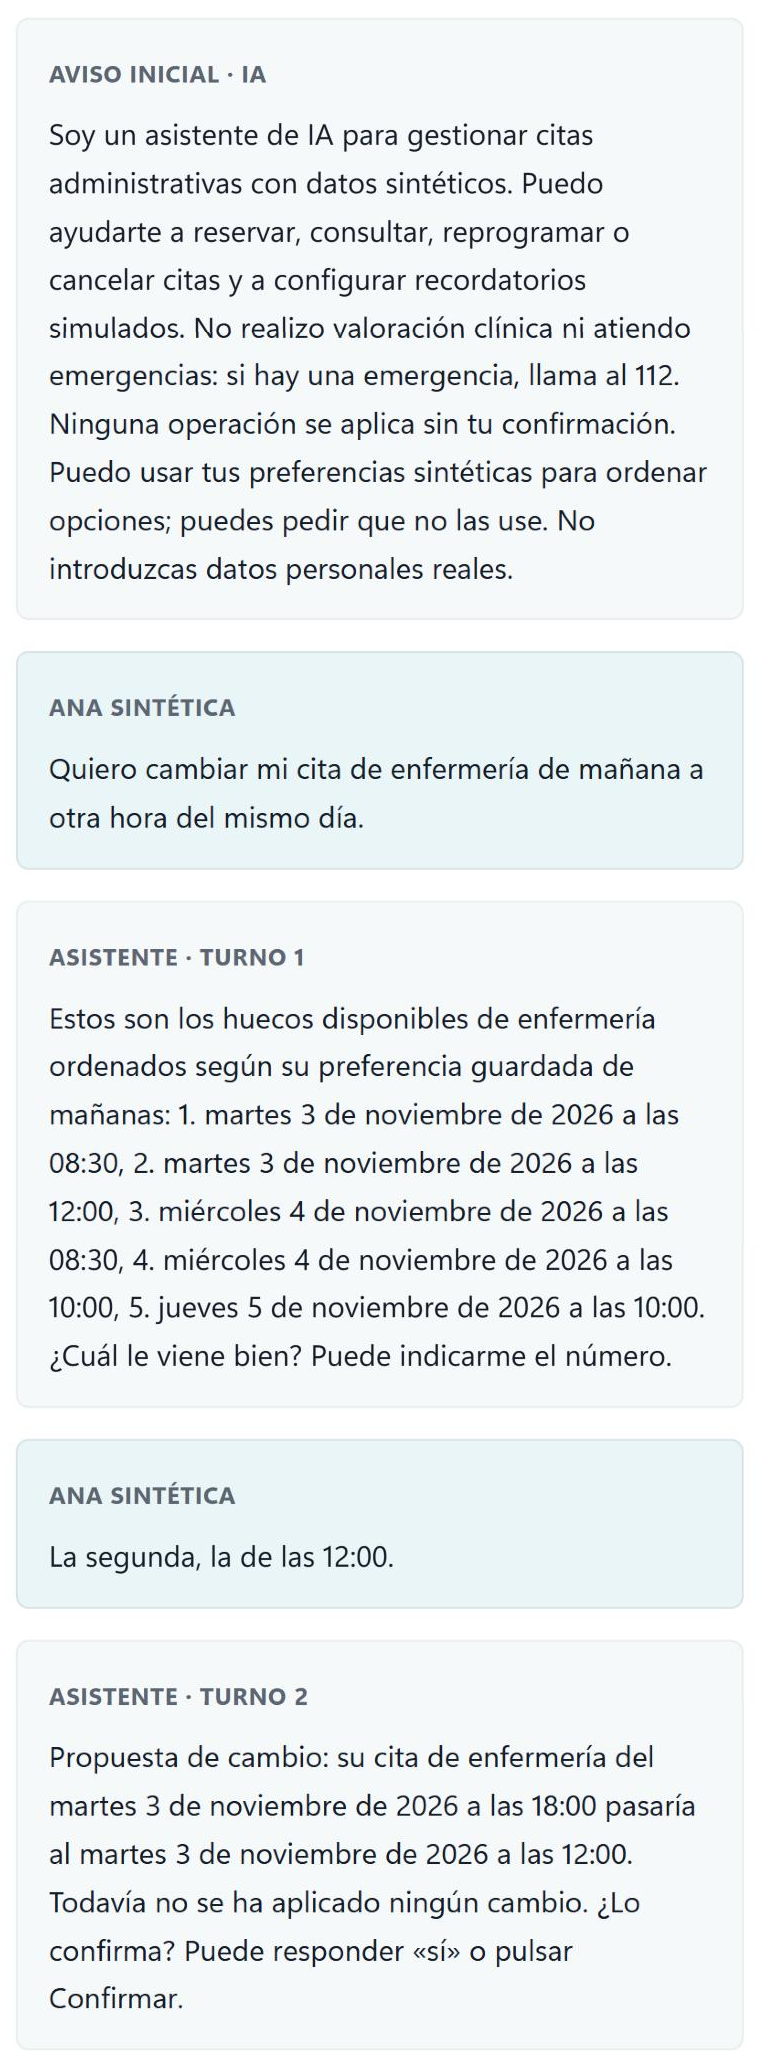
\includegraphics[width=\dimexpr\linewidth-2\fboxrule\relax]{assets/capturas/asistente-propuesta-a.png}}
\end{minipage}%
\hspace{0.04\textwidth}%
\begin{minipage}[t]{0.45\textwidth}
\vspace{0pt}
\fcolorbox{black!25}{white}{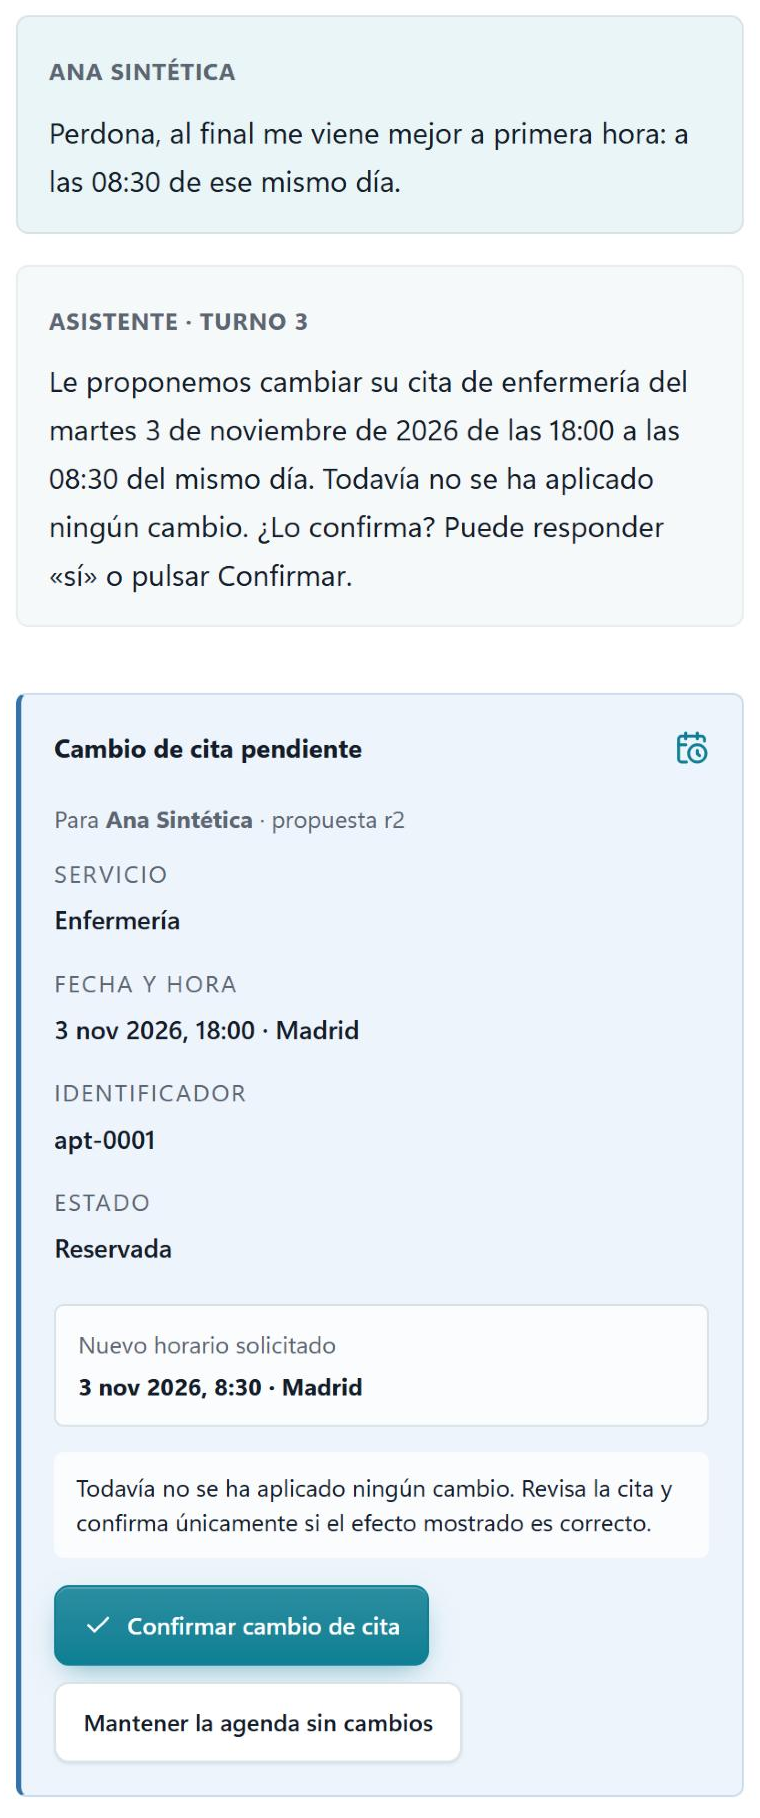
\includegraphics[width=\dimexpr\linewidth-2\fboxrule\relax]{assets/capturas/asistente-propuesta-b.png}}
\end{minipage}
\caption[Cambio de cita negociado en el portal CitaLab]{Cambio de una cita en el
portal CitaLab (M5 con Gemini, datos sintéticos y vista estrecha). A la
izquierda, el aviso inicial identifica al asistente como IA y anuncia que
ninguna operación se aplica sin confirmación. Después, Ana pide mover su cita
de enfermería y el asistente le ofrece los huecos libres, ordenados según su
preferencia guardada de mañanas. Ana elige
uno y recibe una primera propuesta. A la derecha, Ana rectifica la hora antes
de confirmar. El asistente sustituye la propuesta por otra revisión (r2) y la
tarjeta muestra la cita actual y el nuevo horario. La agenda no cambia hasta
pulsar \enquote{Confirmar cambio de cita}. Tras la confirmación, el asistente
informa del cambio y la gestión queda completada.}
\label{fig:portal-propuesta}
\end{figure}

El inspector muestra las llamadas al modelo, las herramientas utilizadas y las
decisiones de política. La sección de evaluación reúne las campañas, las
transcripciones y las comprobaciones de cada episodio. La revisión de las
conversaciones sigue el procedimiento del capítulo~\ref{chap:metodologia-evaluacion}.

La API utiliza sesiones, protección frente a la falsificación de peticiones
entre sitios (CSRF) y roles de administración, revisión y paciente. El acceso de una representante depende de la relación sintética
registrada. No se concede por una afirmación en el diálogo. Los turnos se
procesan de forma asíncrona y se rechazan las solicitudes con un número de
secuencia desfasado para evitar respuestas cruzadas.

Los registros operativos y el historial de investigación tienen finalidades
distintas. Las entradas y salidas completas de las llamadas del portal solo se
conservan cuando se activa el diagnóstico. La administración puede eliminar
el historial y las copias diagnósticas que superen el plazo configurado.

\section{Trazas y consumo}

Cada intento de llamada registra el agente, el modelo, la versión de las
instrucciones, la latencia, los tokens disponibles y el resultado del proveedor.
En la evaluación se conservan además las entradas y salidas necesarias para
examinar el episodio. El consumo del asistente se distingue del correspondiente
al usuario simulado.

Ante errores transitorios, cada llamada admite hasta cuatro intentos, con una espera
exponencial o la indicada en \texttt{Retry-After}, hasta un máximo de 90 segundos. Estas medidas están
orientadas a la evaluación: permiten que una campaña larga resista los fallos
pasajeros del proveedor sin que se cuenten como errores del asistente. Si un
proveedor deja de responder de forma persistente, su cola se detiene y se
reanuda más tarde sin repetir lo completado
(apartado~\ref{sec:metodo-ejecucion}).

El ejecutor guarda cada episodio terminado o interrumpido en disco. Los
reintentos reciben registros y trazas propios. Al reanudar, las conversaciones
completadas se conservan y se continúa con las pendientes y los incidentes
seleccionados para repetir. El manifiesto impide mezclar fuentes o parámetros
distintos dentro de una misma campaña.

\section{Verificación técnica}

Las pruebas automáticas se ejecutan sin llamadas reales a los modelos. Utilizan
respuestas preparadas y transportes simulados para comprobar tanto los recorridos
correctos como las situaciones de error.

En la agenda se prueban la idempotencia, los conflictos de disponibilidad,
las versiones de los recursos y la conservación de la cita cuando falla una
reprogramación. Las pruebas de políticas comprueban el acceso a datos propios,
la representación, la confirmación de propuestas y las vistas del perfil.
También se incluyen solicitudes con identificadores inventados, confirmaciones
en forma de pregunta y operaciones sobre recursos ajenos.

Las pruebas del asistente recorren M5, S1 y H con información incompleta,
correcciones y respuestas que anuncian efectos inexistentes. Las del portal
comprueban sesiones, permisos, aislamiento de conversaciones y retención.
En la evaluación se verifica la coherencia de los casos con sus agendas, el
oráculo y el análisis. La recuperación se prueba con errores de cuota,
interrupciones del simulador, continuidad de las otras colas y reanudación sin
sobrescribir los intentos guardados.
